% \paragraph{Summary}

We have developed a novel Bayesian nonparametric model for spike sorting called \smug.  Our model and inference procedure incorporate certain features that previous approaches---be they nonparametric or not---lacked.  Most importantly, we developed a variational Bayesian online inference scheme, that enabled faster than real-time posterior inference.  Such computational efficiency is crucial for sequential experimental design \cite{}.  Although we only provided our algorithm with streaming data, \smug\ outperformed all competitor \emph{batch} algorithms (that is, algorithms that consume all the data at once). Our improved sensitivity and specificity seem to arise from multiple sources including (i) improved detection, (ii) correlated noise, (iii) capturing overlapping spikes, (iv) tracking waveform dynamics, and (v) utilizing multiple channels.  While others have developed closely related Bayesian models for clustering \cite{WoodBla2008,wood2009}, deconvolution based techniques \cite{Pillow2013}, time-varying waveforms \cite{calabrese2011kalman},  \emph{or} online methods \cite{OSORT, Franke2010}, we are the first to our knowledge to incorporate \emph{all} of those features.

An interesting implication of our work is that it seems that our errors may be irreconcilable using merely first order methods, that is, methods that only consider the mean waveform to detect and cluster.  Fig.\ \ref{fig:IC-PCA} (left) shows the mean waveform for the true positives, missed positives, and false positives.  The means of the true and false positives are essentially identical, suggesting that even in the full 30-dimensional space excluding those waveforms from being estimates spikes would be difficult.  Projecting each waveform into the first two PCs is similarly suggestive, as the missed positives do not seem to be in the cluster of the true positives. Thus, in future work, we will explore dynamic and multiscale dictionaries \cite{ChenMaggioni12}, as well as incorporate a more rich history and stimulus dependence.  
Moreover, although our algorithm is linear in time, the slope depends on the number of channels (see Supp.\ Fig. \ref{fig:timing}).  Fortunately, embarrassingly parallel implementations of this method, using one node per multitrode, is straightforward.  The addition of these features to \smug\ will hopefully create an enabling technology to  simultaneously measure neural activity from many thousands of neurons---while adapting the stimulus optimally---to further unlock the mysteries of the brain.



\begin{center}
\begin{SCfigure}[3]
	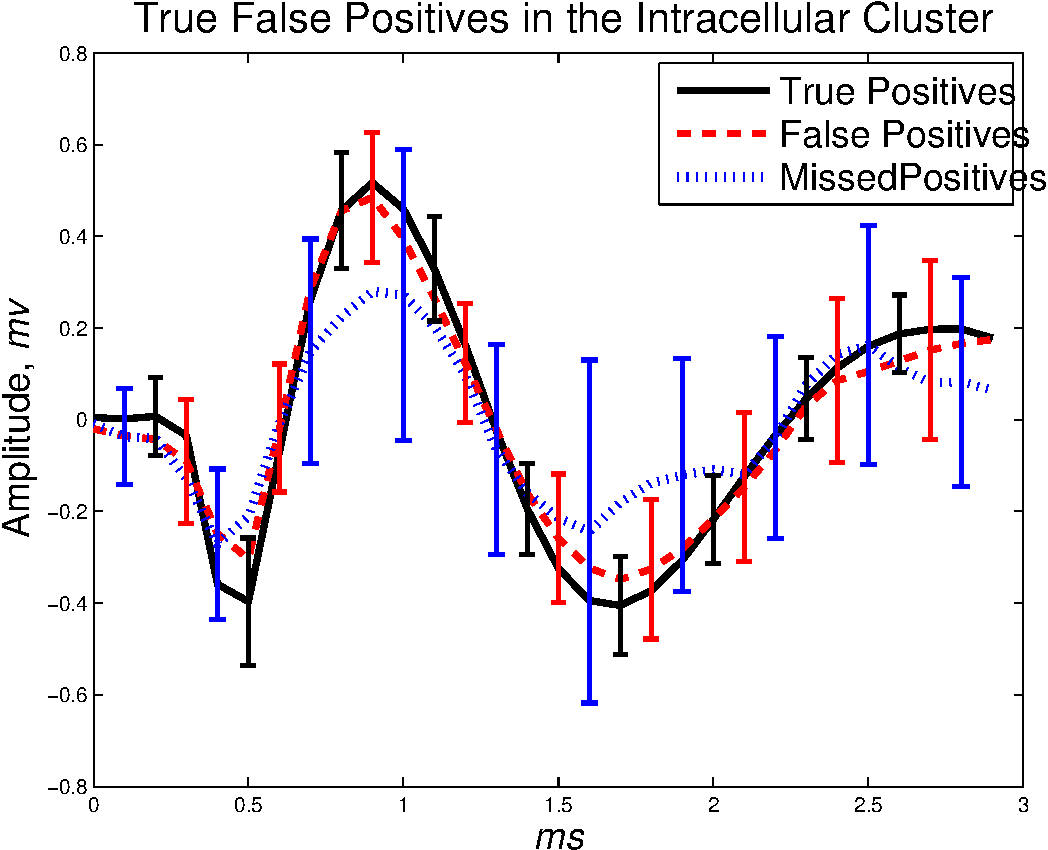
\includegraphics[width=.3\textwidth]{../figs/IntracellularTrueFalsePositivesv2}
	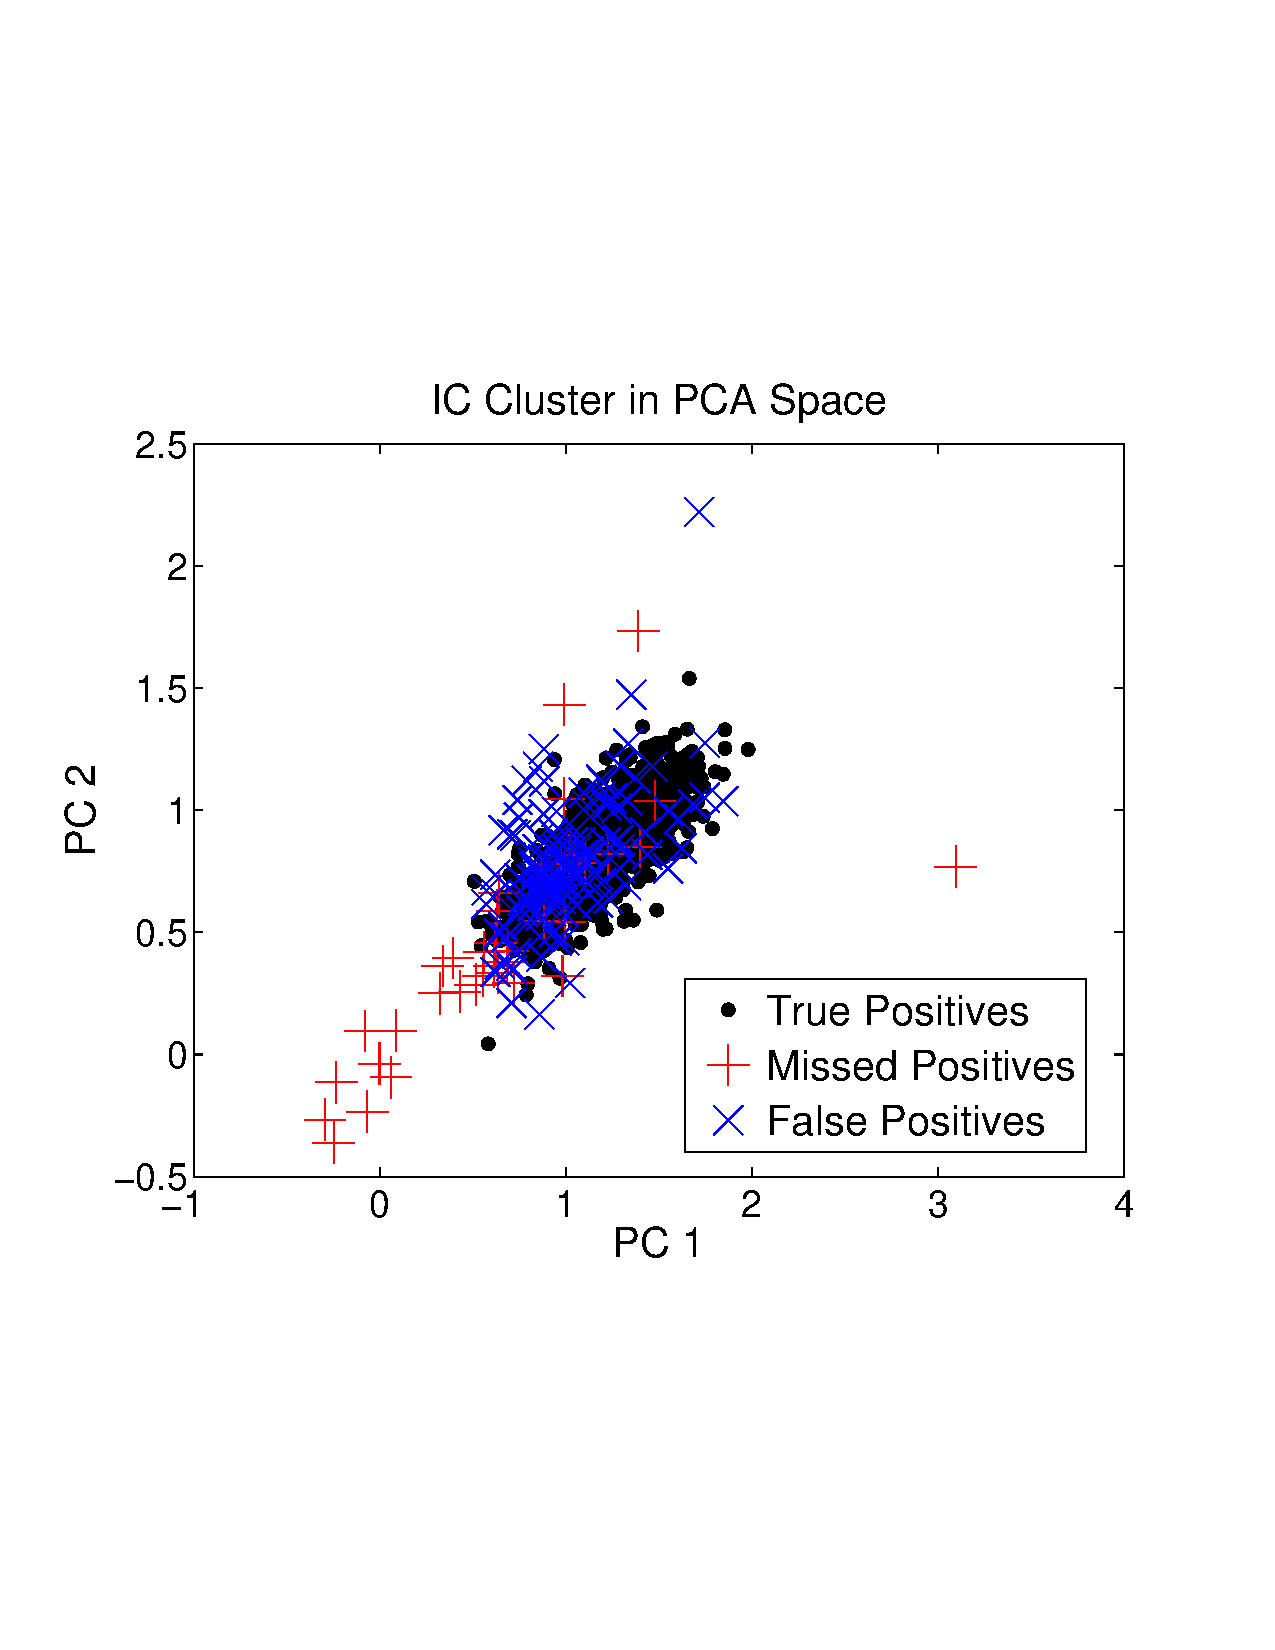
\includegraphics[width=.3\textwidth]{../figs/new/ICclusteroldpca.pdf}
% 		\begin{subfigure}[b]{.33\textwidth}
% 	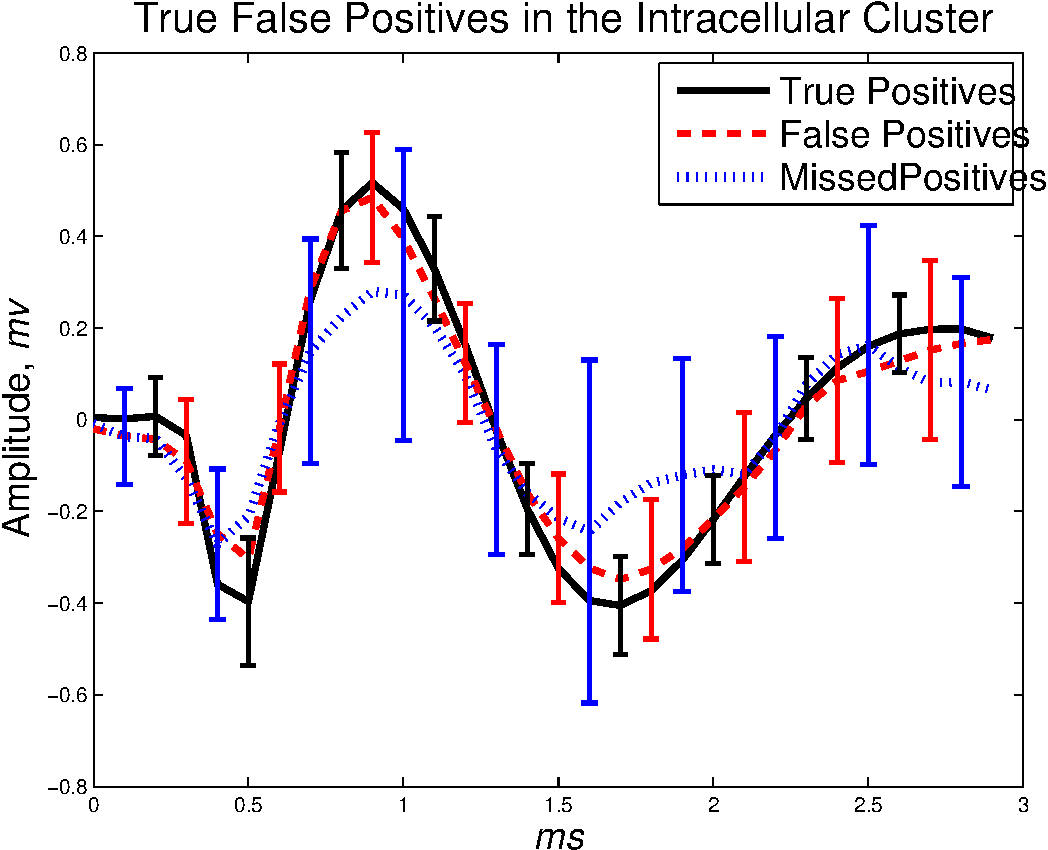
\includegraphics[width=\textwidth]{../figs/IntracellularTrueFalsePositivesv2}
% 	\caption{}
% 	\label{truewaveforms}
% 	\end{subfigure}
% \begin{subfigure}[b]{.33\textwidth}
% 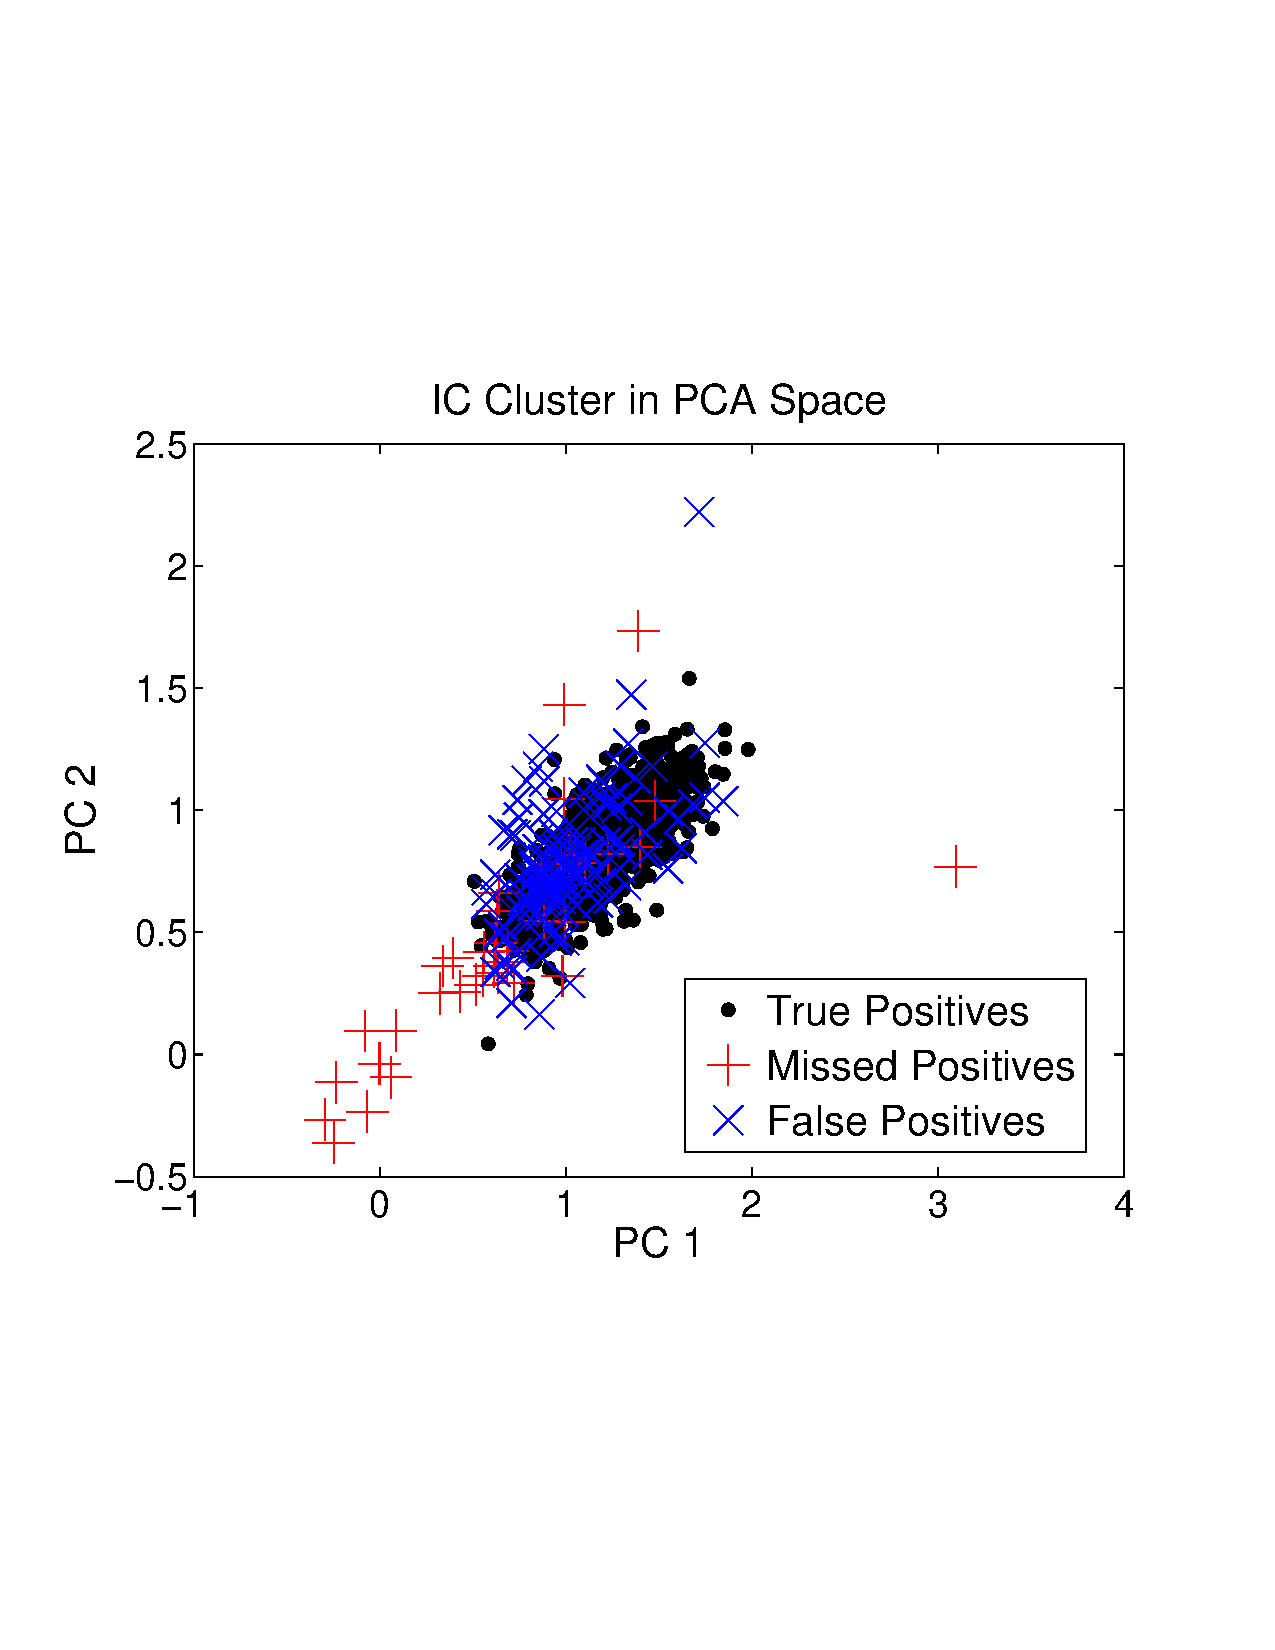
\includegraphics[width=\textwidth]{../figs/new/ICclusteroldpca.pdf}
% \caption{}
% \label{fig:ICold}
% \end{subfigure}
% \begin{subfigure}[b]{.33\textwidth}
% 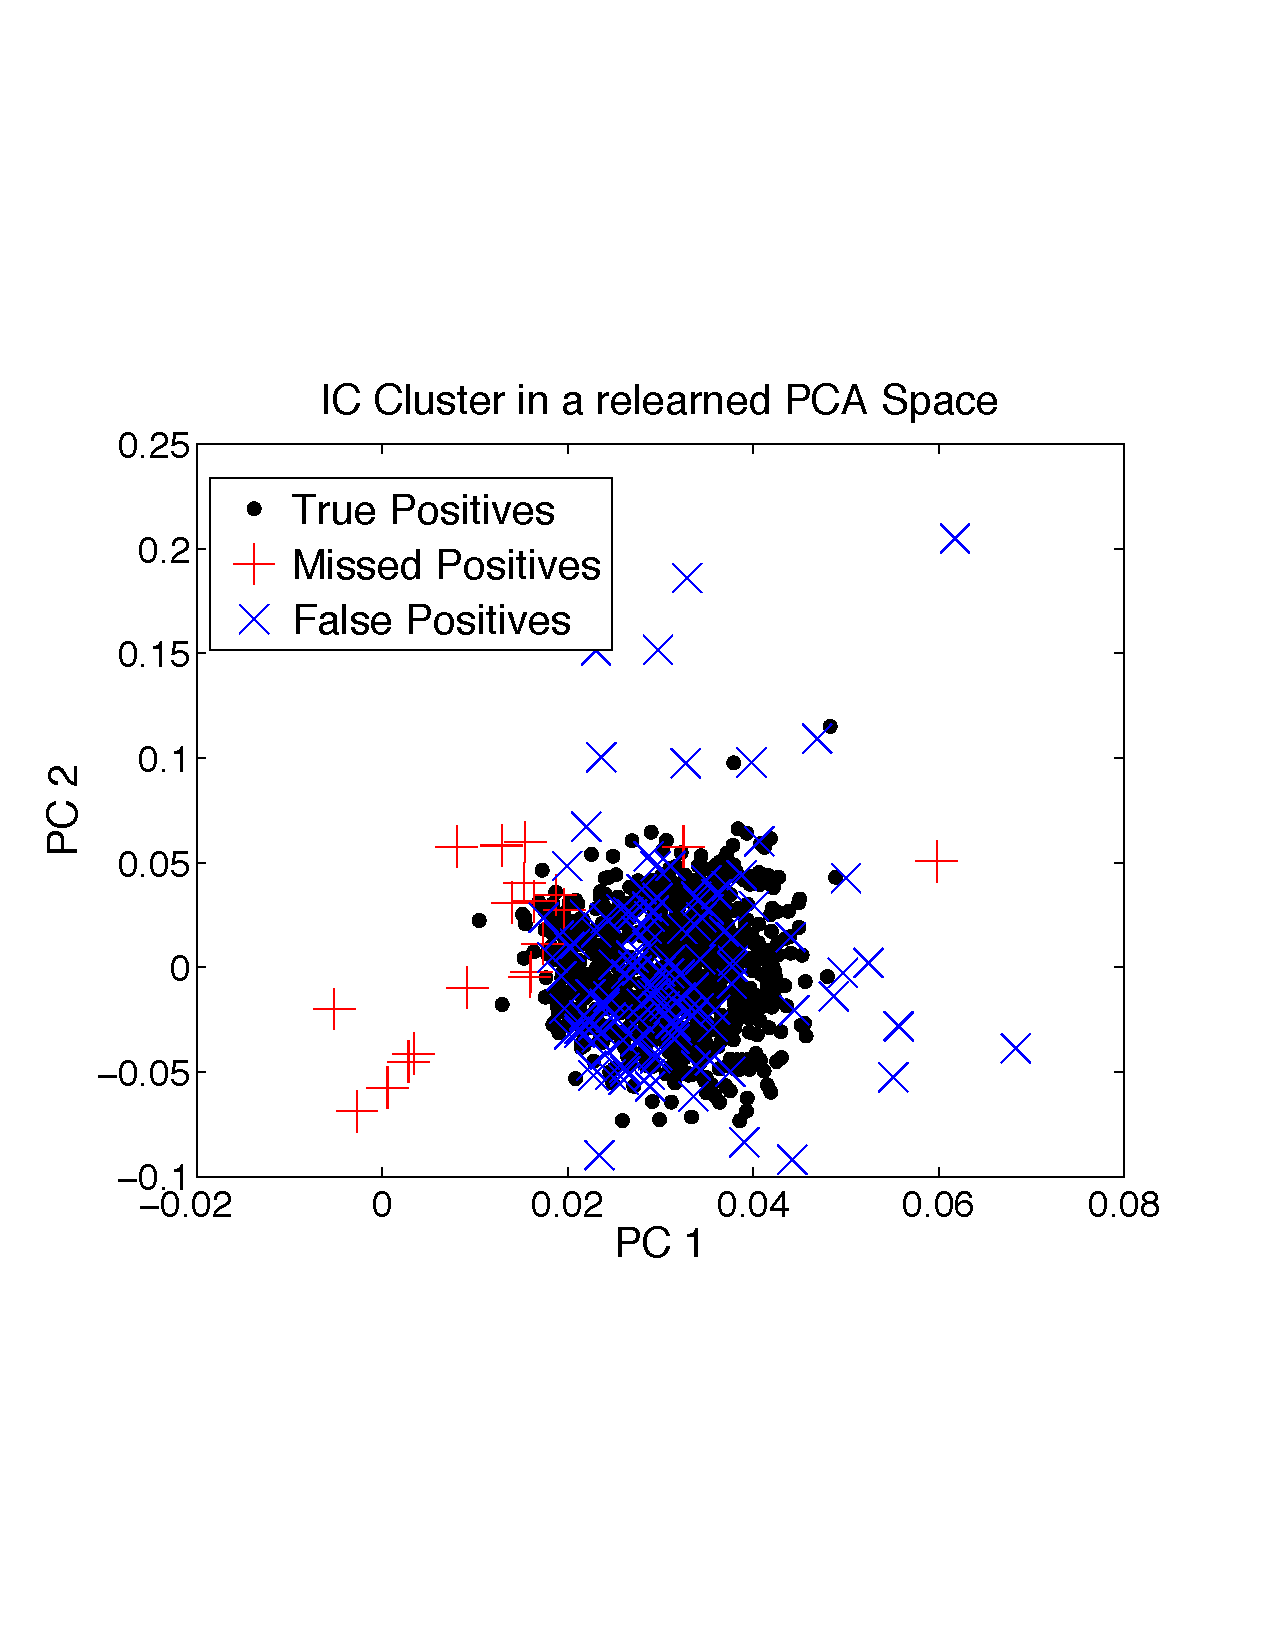
\includegraphics[width=\textwidth]{../figs/new/ICclusternewpca.pdf}
% \caption{}
% \label{fig:ICnew}
% \end{subfigure}
\caption{
Template matching.
(c) Errorbar plots of the true positives and the false positives in the IC cluster.  While the false positives have slightly more variability, the mean shape for the false positives and the true positives is nearly identical.  The true misses have a significantly lower amplitude as well as high variability. 
} \label{fig:IC-PCA}
\end{SCfigure}
\end{center}



% 
% in discussion:
% 
% embarrassingly parallel per 4
% 
% ignore time steps that aren't useful
% 
% let $\lambda_i$ vary as a function of: (i) spike histories, (ii) stimulus, (iii) possibly baseline drift?
% 
% 
% \clearpage
% \section{comments}
% 
% {\color{red} perhaps add comments about time-evolution and the false positives we avoid by using multi-channel analysis}
% 
% \jovo{add grids to all panels of all figs by default, remove if it looks shitty.}
% 
% \jovo{@dec - for fig 1 keep colors/symbols the same in the two panel, if possible.  maybe use a scheme where color indicates algorithm and shape indicates \# of components.  also, be consistent about "IC" cluster vs. "Intracellular" Cluster. and normalize, renaming axes XY Rate instead of only XY. (b) title should be ``ROC Curve Comparisons''}  
% 
% 
